\chapter{Modeling techniques for SAF microarchitectures}
\label{chapter:modeling}

This section will introduce the overarching modeling strategy employed in this work, tying together energy, area and workload modeling into a single scheme. The following considerations are relevant:

\begin{itemize}
    \item Recall from Chapter~\ref{chapter:conceptual_framework} that one of the goals of this work is to associate SAF microarchitecture primitives with analytical cost models (i.e. models of energy and area.) Toward that end, Chapter~\ref{chapter:rtl} introduced a number of RTL designs which were developed and characterized for this work.
    \item However, we still need a way to convert RTL characerization results, into SAF microarchitecture primitive models with well-defined energy-per-action and area.
    \item Also recall from Chapter~\ref{chapter:conceptual_framework} that another goal of this work is to decouple SAF microarchitecture from architecture and dataflow. As shown in Figure~\ref{fig:sparse_sbuff_wkld_overview}, we hope to encapsulate all details of architecture and dataflow behind format interfaces with well-defined measures of workload.
\end{itemize}

Recall that the RTL in Chapter~\ref{chapter:rtl} is parameterized. The power-consumption and area of RTL components will scale with the parameter values. However, more subtly, the \textit{load-handling capability} of the RTL components also scales with the parameter values. For example, a naive two-finger-merge-based intersection unit will be able to intersect more input operands per cycle, if it is constructed with a greater degree of input vectorization; or, a prefix sum unit designed for operands which have some number of bits, will be able to support operands with a larger range of possible values if the number of bits is increased. Thus RTL parameters represent a tradeoff between cost (power, area) and load-handling capability; going forward these parameters will be referred to as \textit{scale parameters.}

The motivation for assigning a measure of workload to each format interface at the outset, is so that the scale parameters of the SAF microarchitecture may be tuned properly. The SAF microarchitecture scale parameters should be set such that

\begin{itemize}
    \item The SAF microarchitecture can process sparse format metadata at the rate which it is being served over the format interface by the smartbuffer.
    \item The SAF microarchitecture is capable of serving processed outputs back to the buffer via the format interface, at the rate which the buffer was designed for.
\end{itemize}

Failure to meet either of the above requirements should in principle lead to a slowdown in the whole design.

Before we can perform SAF microarchitecture design-space exploration, we first require SAF microarchitecture models. Otherwise comparison between SAF microarchitecture designs is impossible.

This section will introduce (1) the structure of energy/area models developed in this work, (2) a method for modeling SAF microarchitecture workloads in sparse tensor accelerators, and (3) a process for scaling up the SAF microarchitecture to match the magnitude of the workload imposed upon it.

\begin{figure}[h]
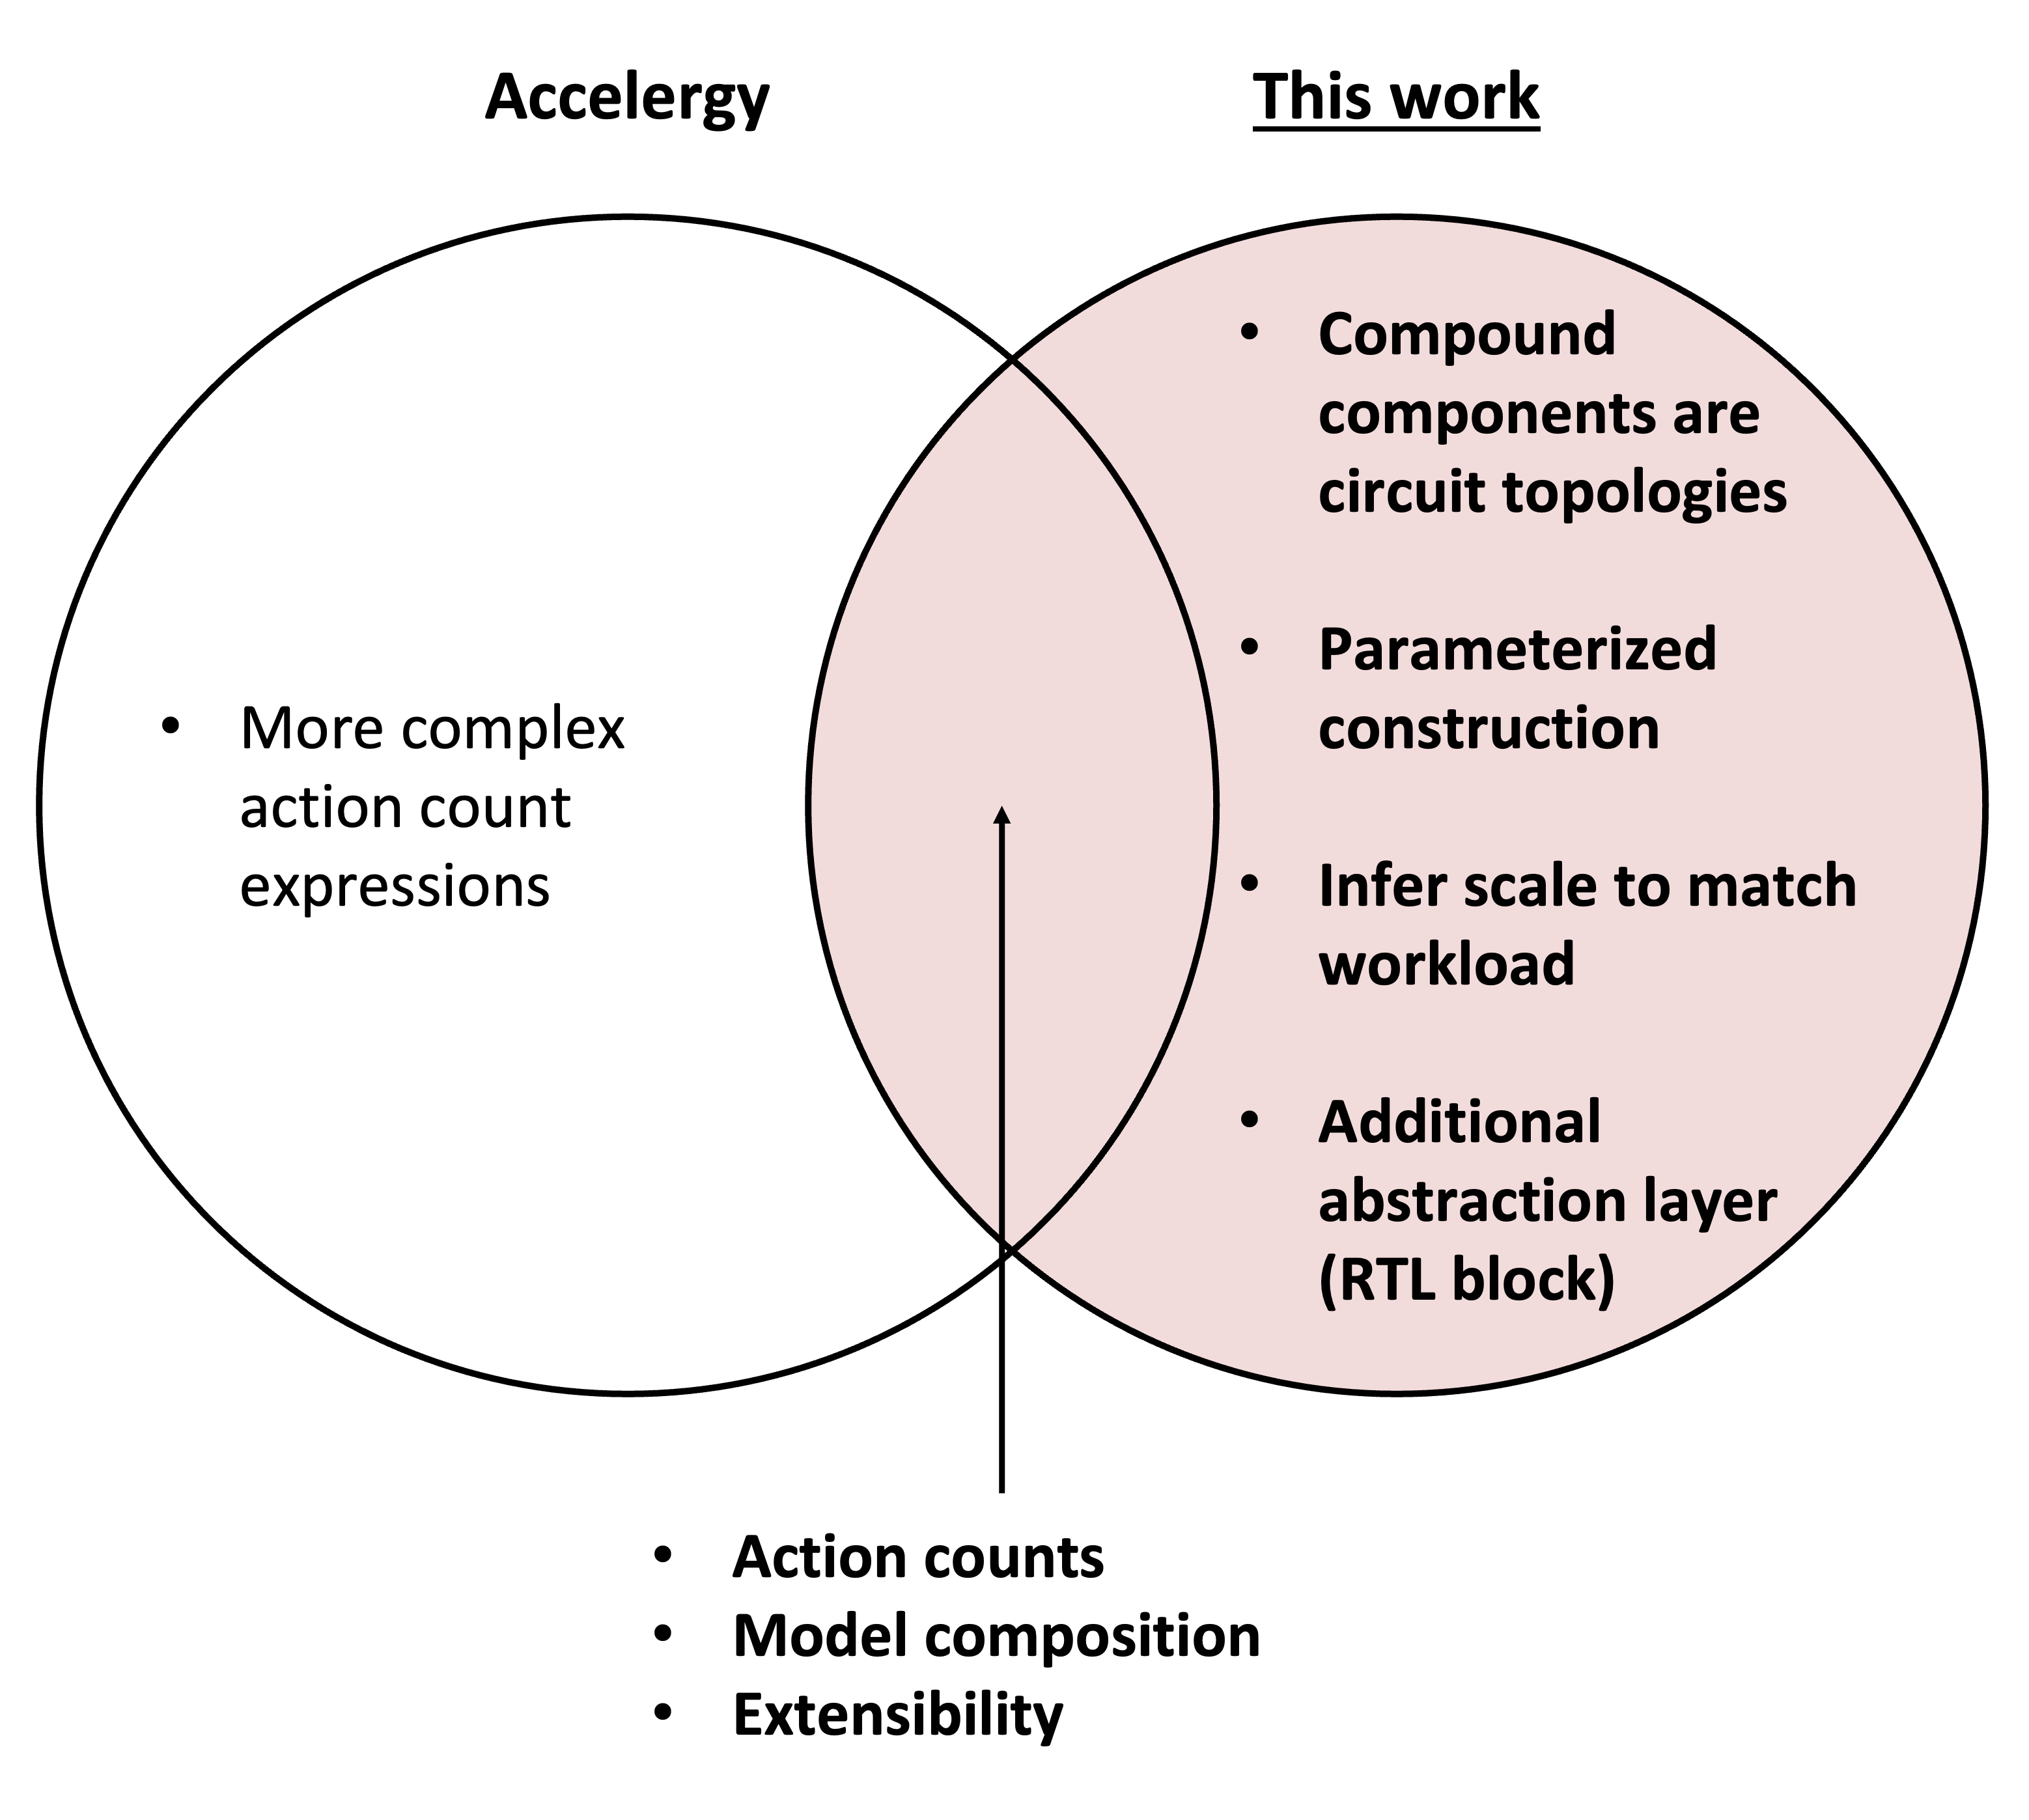
\includegraphics[width=\textwidth]{figures/accelergy_comparison.png}
\caption{The Accelergy modeling framework compared to the modeling framework in this work.}
\label{fig:accelergy_comparison}
\end{figure}

\section{Utilizing SAF microarchitecture modeling for tradeoff decisions}



One challenge is that taxonomic design-space exploration yields high-level topologies but does not address low-level optimization of the microarchitecture. Ideally each SAF primitive's action-energy and area models reflect good design choices which minimize energy and area as nearly as possible; the problem is that the workload (or just ``load'') of sparse format processing work is highly dependent on where a SAF microarchitecture resides within an architecture; load-handling requirements lower-bound the cost of designing sufficiently performant SAF microarchitectures.

To that end, this section:

\begin{itemize}
    \item Develops a multi-dimensional model of the \textit{load} placed upon SAF microarchitectures
    \item Develops a conceptual framework for parameterizing SAF microarchitecture \textit{load-handling capability}
    \item Shows how to ``solve'' for energy/area models of optimized SAF microarchitectures by solving a constrained mixed-integer non-linear programming problem (MINLP). The optimization constraints are derived by applying load-modeling, circuit-modeling and composition rules to the microarchitecture topology derived from taxonomic design-space exploration
\end{itemize}

\subsection{Load modeling}

It is necessary to have an effective means of characterizing the load that is placed upon a SAF microarchitecture, as well as that component's load-handling capability. Here, load refers to the quantity of work that is imposed upon a microarchitecture, by some appropriate measure, and load-handling capability refers to the threshold load value at which a load becomes unmanageable by a particular microarchitecture. An accurate energy/area model of a microarchitecture must incorporate the insight that greater load-handling capability tends to correlate with a larger and/or more energetically costly microarchitecture\footnote{Note that while SAF microarchitecture energy-per-cycle necessarily increases when the load processed per cycle increases, the \textit{efficency} (energy-per-load-unit) may have a more complex relationship to the load-handling requirement and the microarchitecture characteristics.}.

This section describes
\begin{itemize}
\item A multi-dimensional measure of the load that architectural buffers and arithmetic units impose on SAF microarchitectures
\item A multi-dimensional measure of the load-handling capability of SAF microarchitectures
\item A process of solving for the \textit{minimum load-handling capability requirement} which each SAF microarchitecture must be designed for
\end{itemize}

The area and action-energy of each SAF microarchitecture will scale as a function of load-handling requirements; therefore, solving for minimum load-handling capability requirements is a pre-requisite for exporting analytical energy/area models.

On first blush, it might seem appropriate to use a single scalar quantity to characterize both load and load-handling capability of a component. For example, the \textit{throughput} (number of inputs processed per time) would seem like a good candidate for measuring load and load-handling requirements (since FLOPs is a common compute performance metric.)

However, it quickly becomes apparent that load and load-handling ability are multi-dimensional; what follows is a list of factors which influence loading and load-handling requirements:

\begin{itemize}
    \item \textbf{Word-width.} A microarchitecture capable of handling the throughput imposed by some workload, may nonetheless be unsuitable if i.e. the microarchitecture is expected to process sparse format metadata possessing a greater bitwidth than what the microarchitecture was designed for. Thus, word-width is a dimension of load, and the upper limit on word-width is a dimension of load-handling capability for a particular component.
    \item \textbf{Size of abstract dense rank which underlies a sparse fiber.} Consider a bitmask intersection unit, as employed in the SparTen accelerator paper \cite{sparten}. The degree of parallelism of the bitmask intersection unit microarchitecture is not a function of the throughput of metadata nor of the number of bits in a metadata word (which is in fact equal to one for bitmask format), but rather the parallelism must meet or exceed the cardinality of the abstract dense ranks which underly the sparse fibers being intersected. Thus, the cardinality of the dense rank which underlies a sparse fiber is a dimension of the load on the microarchitecture. The parallelism of the bitmask intersection unit exemplifies a dimension of the microarchitecture's load-handling capability, specifically an upper-limit on dense rank cardinality which the microarchitecture can handle.
    \item \textbf{Memory access width.} The SAF microarchitecture must be able to receive sparse format metadata in chunks equal to the memory's access bitwidth - i.e., for metadata with a bitwidth of 4 stored in a memory with 8-bit-wide reads, up to two metadata words may be made available to the SAF microarchitecture per access, worst-case. If the SAF microarchitecture only needs to read format metadata a few times over many cycles, then the latency of sequentially processing multiple metadata words can be hidden inside the time between wide reads. However, a SAF microarchitecture that is making wide memory accesses every cycle cannot hide the latency of sequential processing and thus requires a (probably more costly) SIMD design. This motivates memory access width as a dimension of load and load-handling capability.
    \item \textbf{Local architectural throughput.} Suppose that an architecture uses a SIMD MAC unit capable of 4x $C = C + A \times B$ operations per cycle to compute an inner-product; let's define $4$ MACs/cycle as the \textit{arithmetic throughput requirement.} To avoid MAC underutilization, the arithmetic throughput requirement in turn poses requirements on the whole design; for example, four $A$ and four $B$ operands per cycle are read from the $A$ and $B$ buffers respectively. 

    % Radix-2 intersection example figure
    \begin{figure}[H]
        \centering
        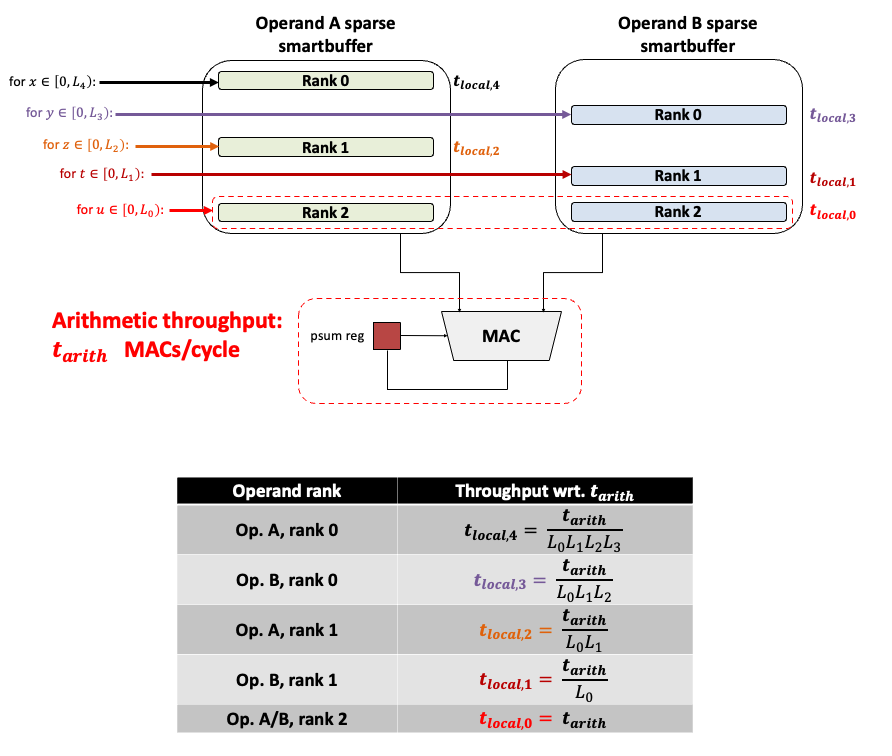
\includegraphics[width=\linewidth]{figures/local_throughput_diagram.png}
        \caption{The local throughput at each rank grows with increasing arithmetic throughput, and shrinks in proportion to the stride of the loop(s) which the fiber is bound to.}
        \label{fig:local_throughput_diagram}
    \end{figure}

    As an optimization, the designer implements a bidirectional skipping SAF between buffers $A$ and $B$. The skipping microarchitecture intersects $A$ and $B$ metadata and outputs a pair of $A$ and $B$ data read addresses for each intersection match. Consider what load-handling requirements the skipping microarchitecture must be designed for, in order to avoid MAC under-utilization: the skipping microarchitecture must serve $4$ $A$ addresses and $4$ $B$ addresses per cycle in order to facilitate reading 4 data values per cycle from each operand. Notably, this is a requirement on the skipping microarchitecture which results directly from the arithmetic throughput-handling design-point.

    Note that in the above example, the skipping microarchitecture, buffers, and MAC are all synchronized with the innermost loop of the mapping loop-nest; this is the fastest loop. Conversely, the outermost loops of the mapping loop-nest have greater latency between loop iterations (i.e. more cycles-per-iteration). Microarchitectures synced to slower loops can maximally exploit latency-hiding to relax throughput-handling requirements by spreading out sequential processing over the time between loop iterations. Microarchitectures synced to faster loops must be capable of handling higher processing throughput without exploiting latency hiding. This state of affairs is summarized in Figure~\ref{fig:local_throughput_diagram}
    
    As a precedent, Sparseloop\cite{sparseloop} assumes that data is pre-tiled to match the loop-nest. Under this assumption there is a reasonably clean mapping from loops in the loop nest to fibers in the fibertree of an operand, and thus a microarchitecture which interacts with fiber $i$ must support the throughput imposed by the corresponding loop in the loop-nest. For example, the inner-most loop must keep pace with the arithmetic throughput-handling requirement imposed by the MAC, so any microarchitecture which interacts with the fiber(s) corresponding to the inner loop must also keep pace with the arithmetic throughput requirement. \textit{All other things being equal}, the microarchitectural throughput-handling requirement decreases monotonically as you ascend hierarchically within a fibertree, because successively higher fibers correspond to successively slower loops. 
    
    Define \textit{local architectural throughput} as the unique throughput requirement for processing a \textit{particular} fiber within a \textit{particular} buffer, owing to the synchronization of the whole architecture with the mapping loop nest. Local architecture throughput is a key dimension of the load which the architecture imposes on a SAF microarchitecture. Consequently, throughput-handling capability is a key design requirement - \textit{but not the only key requirement} - for the SAF microarchitecture.
    
    \item \textbf{Degree of fiber sparsity.} Suppose that a fiber with a bitmask representation format resides in some buffer within an architecture. The local architecture throughput requirement for processing this fiber places a lower bound on how many non-zero fiber payloads must be traversed per cycle.

    Since it is given that the fiber is subject to a bitmask format SAF optimization, a format microarchitecture is required for parsing the metadata format. Based on the programming model developed in this work, the buffer will have several format interface ports to facilitate fiber metadata processing: \textit{md\_out}, \textit{pos\_in}, \textit{at\_bound\_in}. The format microarchitecture's ports are wired to read bitmask metadata from the buffer \textit{md\_out} port, and generate an active-high signal at \textit{at\_bound\_in} to signal when the entire fiber has been processed.

    How do we derive the format microarchitecture throughput-handling requirement from the local architectural throughput requirement associated with the fiber? The local architectural throughput applies to the rate of traversing non-zero payload values within the fiber, and the number of non-zero payloads may be much less than the dense size of the abstract rank associated with the fiber. In contrast, the number of $1$-bit bitmask metadata words matches the dense rank size regardless of how many non-zero payloads the sparse fiber has. Metadata parsing by the format microarchitecture must keep pace with the traversal of non-zero payloads in the fiber, thus if the fiber is 90\% sparse/10\% dense, $10$ $1$-bit bitmask metadata words must be parsed per non-zero data value on average; if the fiber is 99\% sparse/1\% dense, $100$ $1$-bit bitmask metadata words must be parsed per non-zero data value on average.

    More generally, for a bitmask-formatted fiber with local architectural throughput requirement $t_{arch}$ (in payloads/cycle) and a sparsity fraction $s$, the format microarchitecture must support a metadata parsing throughput of

    \[t_{parse} = \frac{1}{1-s}t_{arch}\]

    Of course, this relationship only holds for bitmask representation format. A representation format such as coordinate-payload has one explicit-coordinate metadata value per non-zero payload, thus \[t_{parse} = t_{arch}\]

    The point is, sparsity $s$ matters because it \textit{sometimes} modulates the microarchitectural throughput-handling requirement imposed by a fiber's local architectural throughput, and thus fiber sparsity is a key dimension of load.

\subsection{Loadspaces}
\label{sec:loadspaces}

To concisely and effectively model loading and load-handling capability, this work builds on the concept of \textit{dataspaces} from Timeloop\cite{timeloop}.

To characterize loading, here the concept of a \textit{loadspace} is introduced. Whereas a dataspace captures the different tensor dimensions of an idealized tensor of values, a loadspace is the space of possible value for load dimensions at a particular point within an architecture or microarchitecture.

% Loadspace dimensions
\begin{figure}[H]
    \centering
    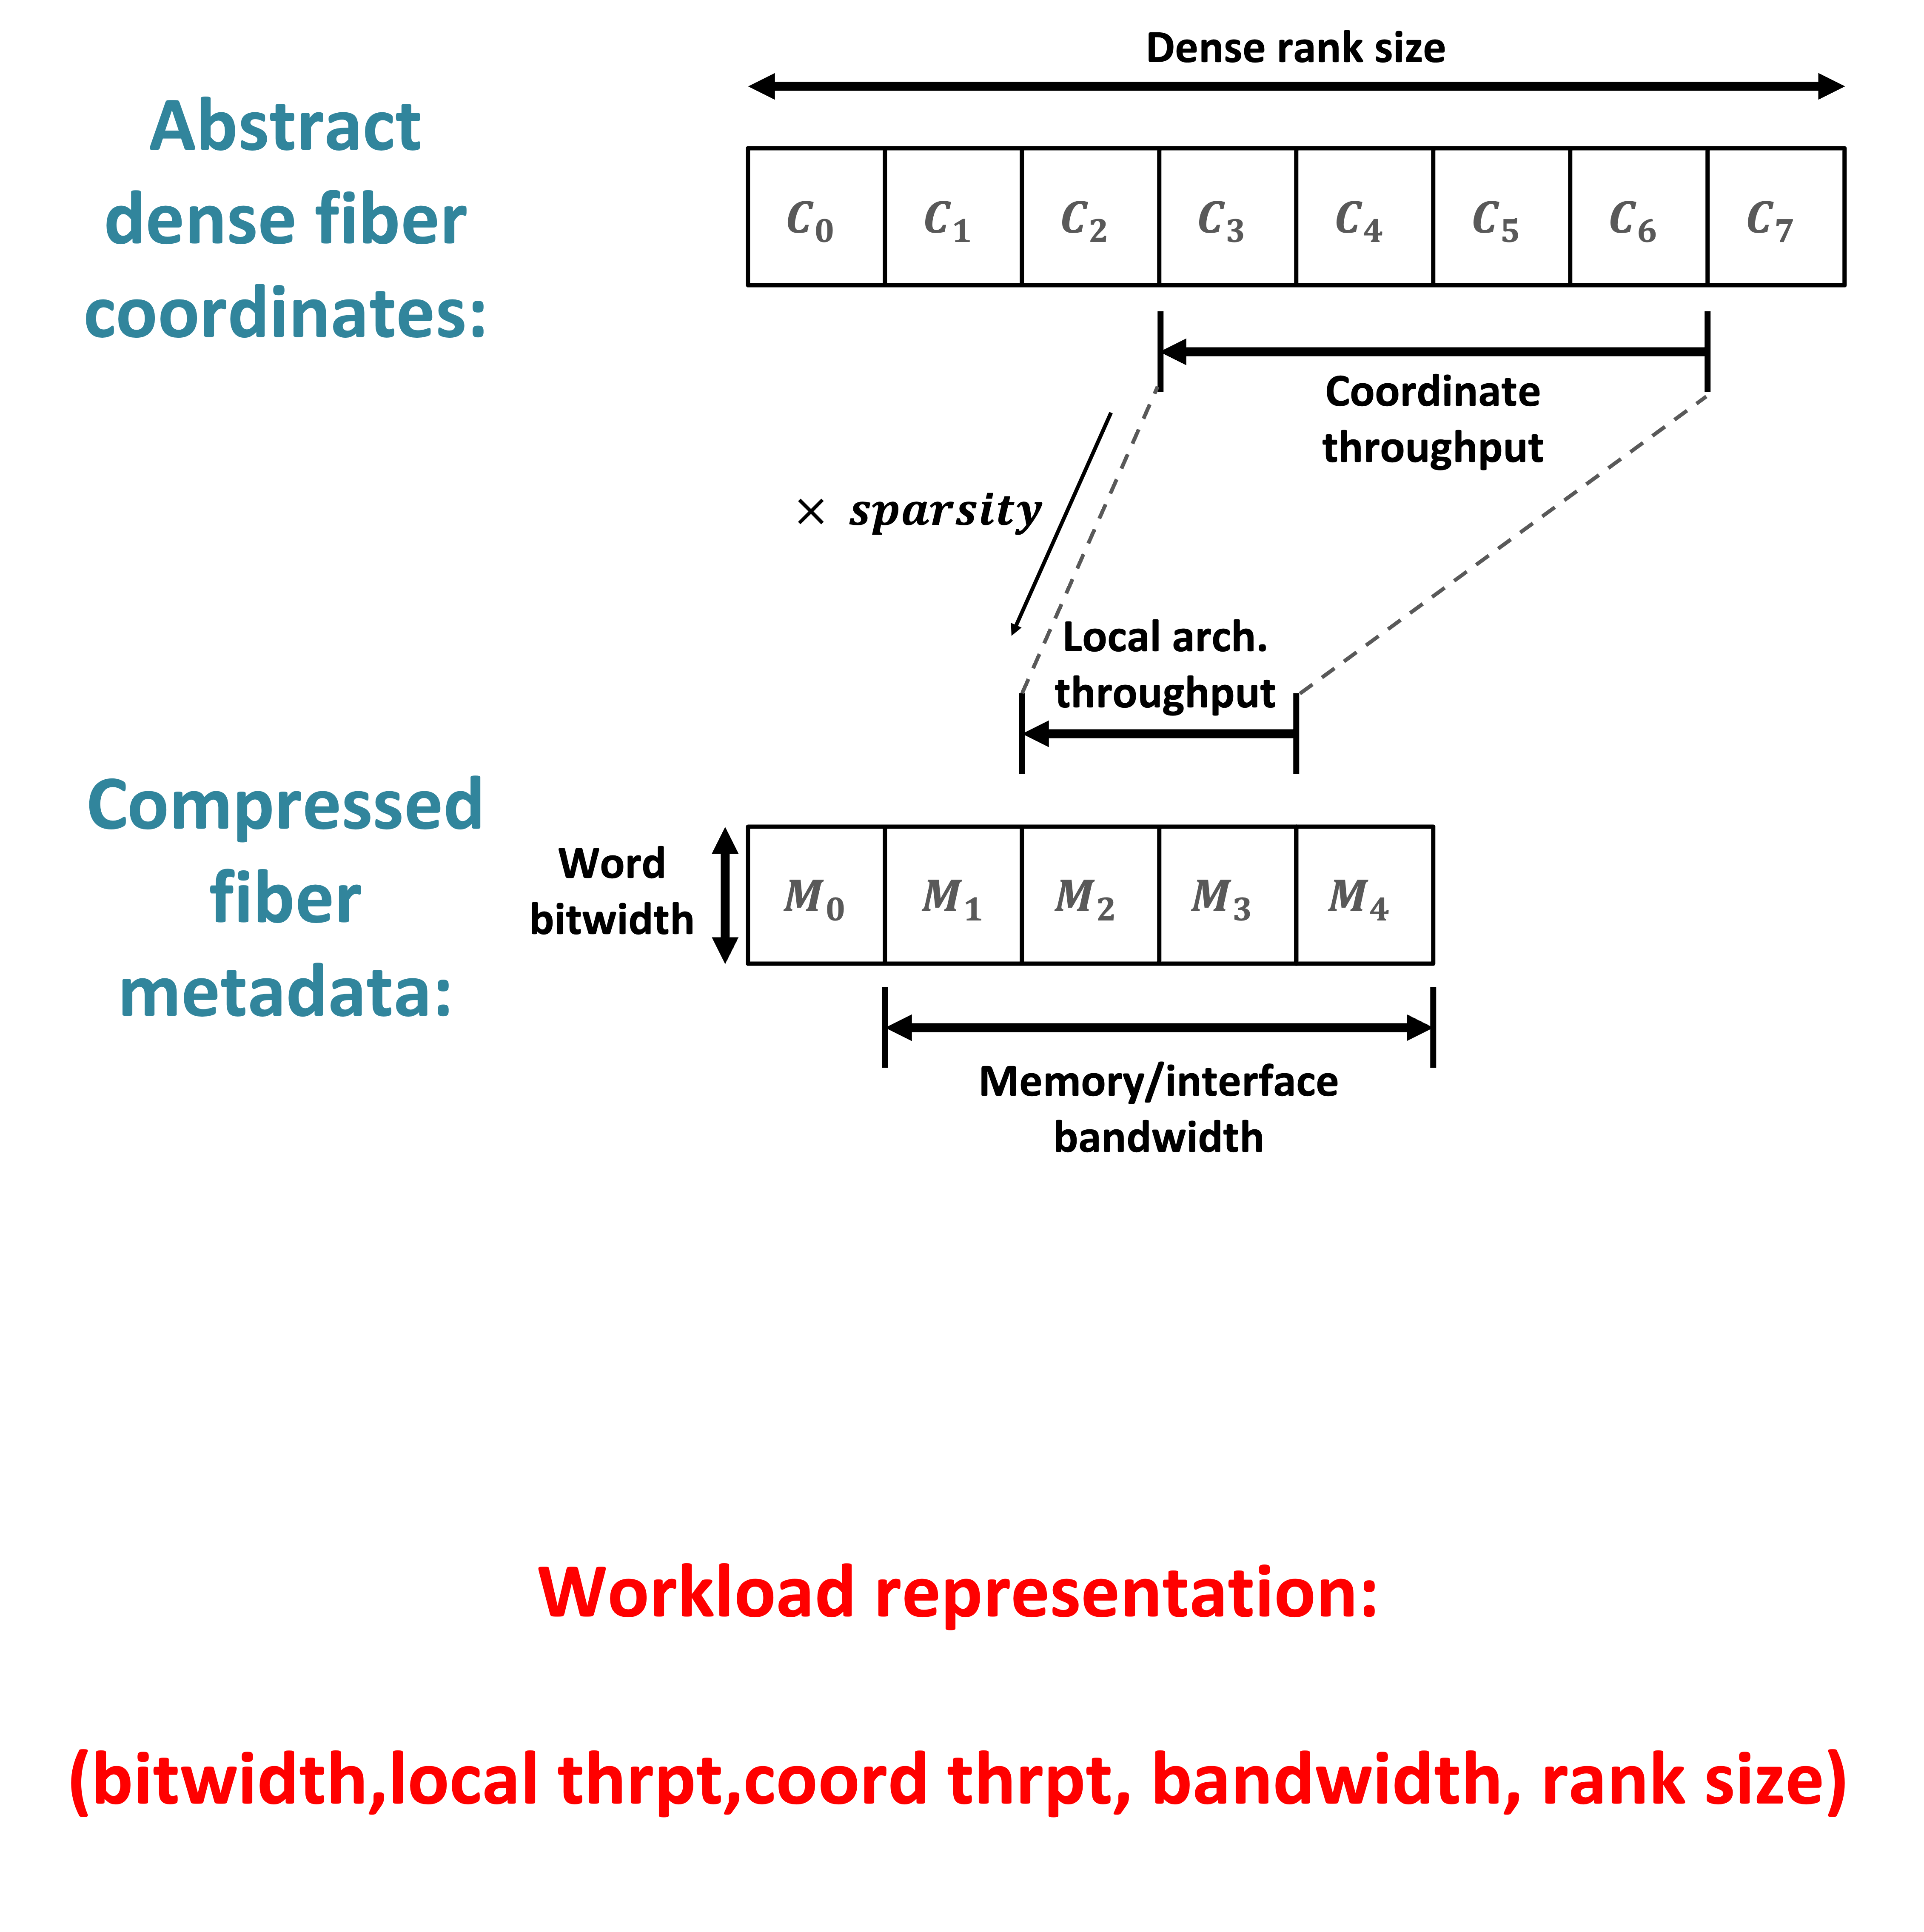
\includegraphics[width=\linewidth]{figures/workload_representation.png}
    \caption{This work proposes modeling workloads as ``loadspaces''. Here, \textit{word bitwidth},  \textit{local architectural throughput}, \textit{coordinate throughput}, and \textit{dense rank size} are proposed as key loadspace dimensions when designing SAF microarchitectures.}
    \label{fig:workload_representation}
\end{figure}

    \begin{table}[h]
        \centering
        \caption{Mnemonics for workload dimensions.}
        \label{table:workload_dimension_mnemonics}
        \begin{tabular}{||c|c|c|c||}
            \hline \hline
            Workload Dimension & Mnemonic & Stands for & Units \\
            \hline \hline
            Dense rank size & nc & num. coordinates & Coordinates \\
            \hline
            Local throughput & pr & position rate & Words/Cycle \\
            \hline
            Sparsity & sp & sparsity & \% \\
            \hline
            Bitwidth & ww & word width & Bits \\
            \hline
            Bandwidth & bw & read width & Bits \\
            \hline \hline
        \end{tabular}
    \end{table}

\subsection{Scalespaces}

As for modeling load handling capability, a good starting point is to note that we ultimately seek to minimize certain objective functions such as energy and area. And the modeling of these objective functions will be based on characterizing certain discrete RTL components. And these RTL components typically have a set of parameters such as data width, parallelism, etc.

Thus, analogous to load spaces, we need a way to capture the different dimensions of the load handling capability, and so we introduce scale spaces which have a dimension for each different parameter that determines the characterized energy or area of the component.

Now we can see how scale spaces and load spaces together allow us to define or solve problems in energy and area modeling. So if we consider a microarchitecture with a scale space that has two ranks and connected to a set of interfaces that collectively have a load space with two ranks,

Each point in the scale space is thus associated with a different energy area combination of values derived from characterization of the RTL .

\subsection{Specifying a SAF microarchitecture primitive model}

\begin{figure}[ht]
    \centering
    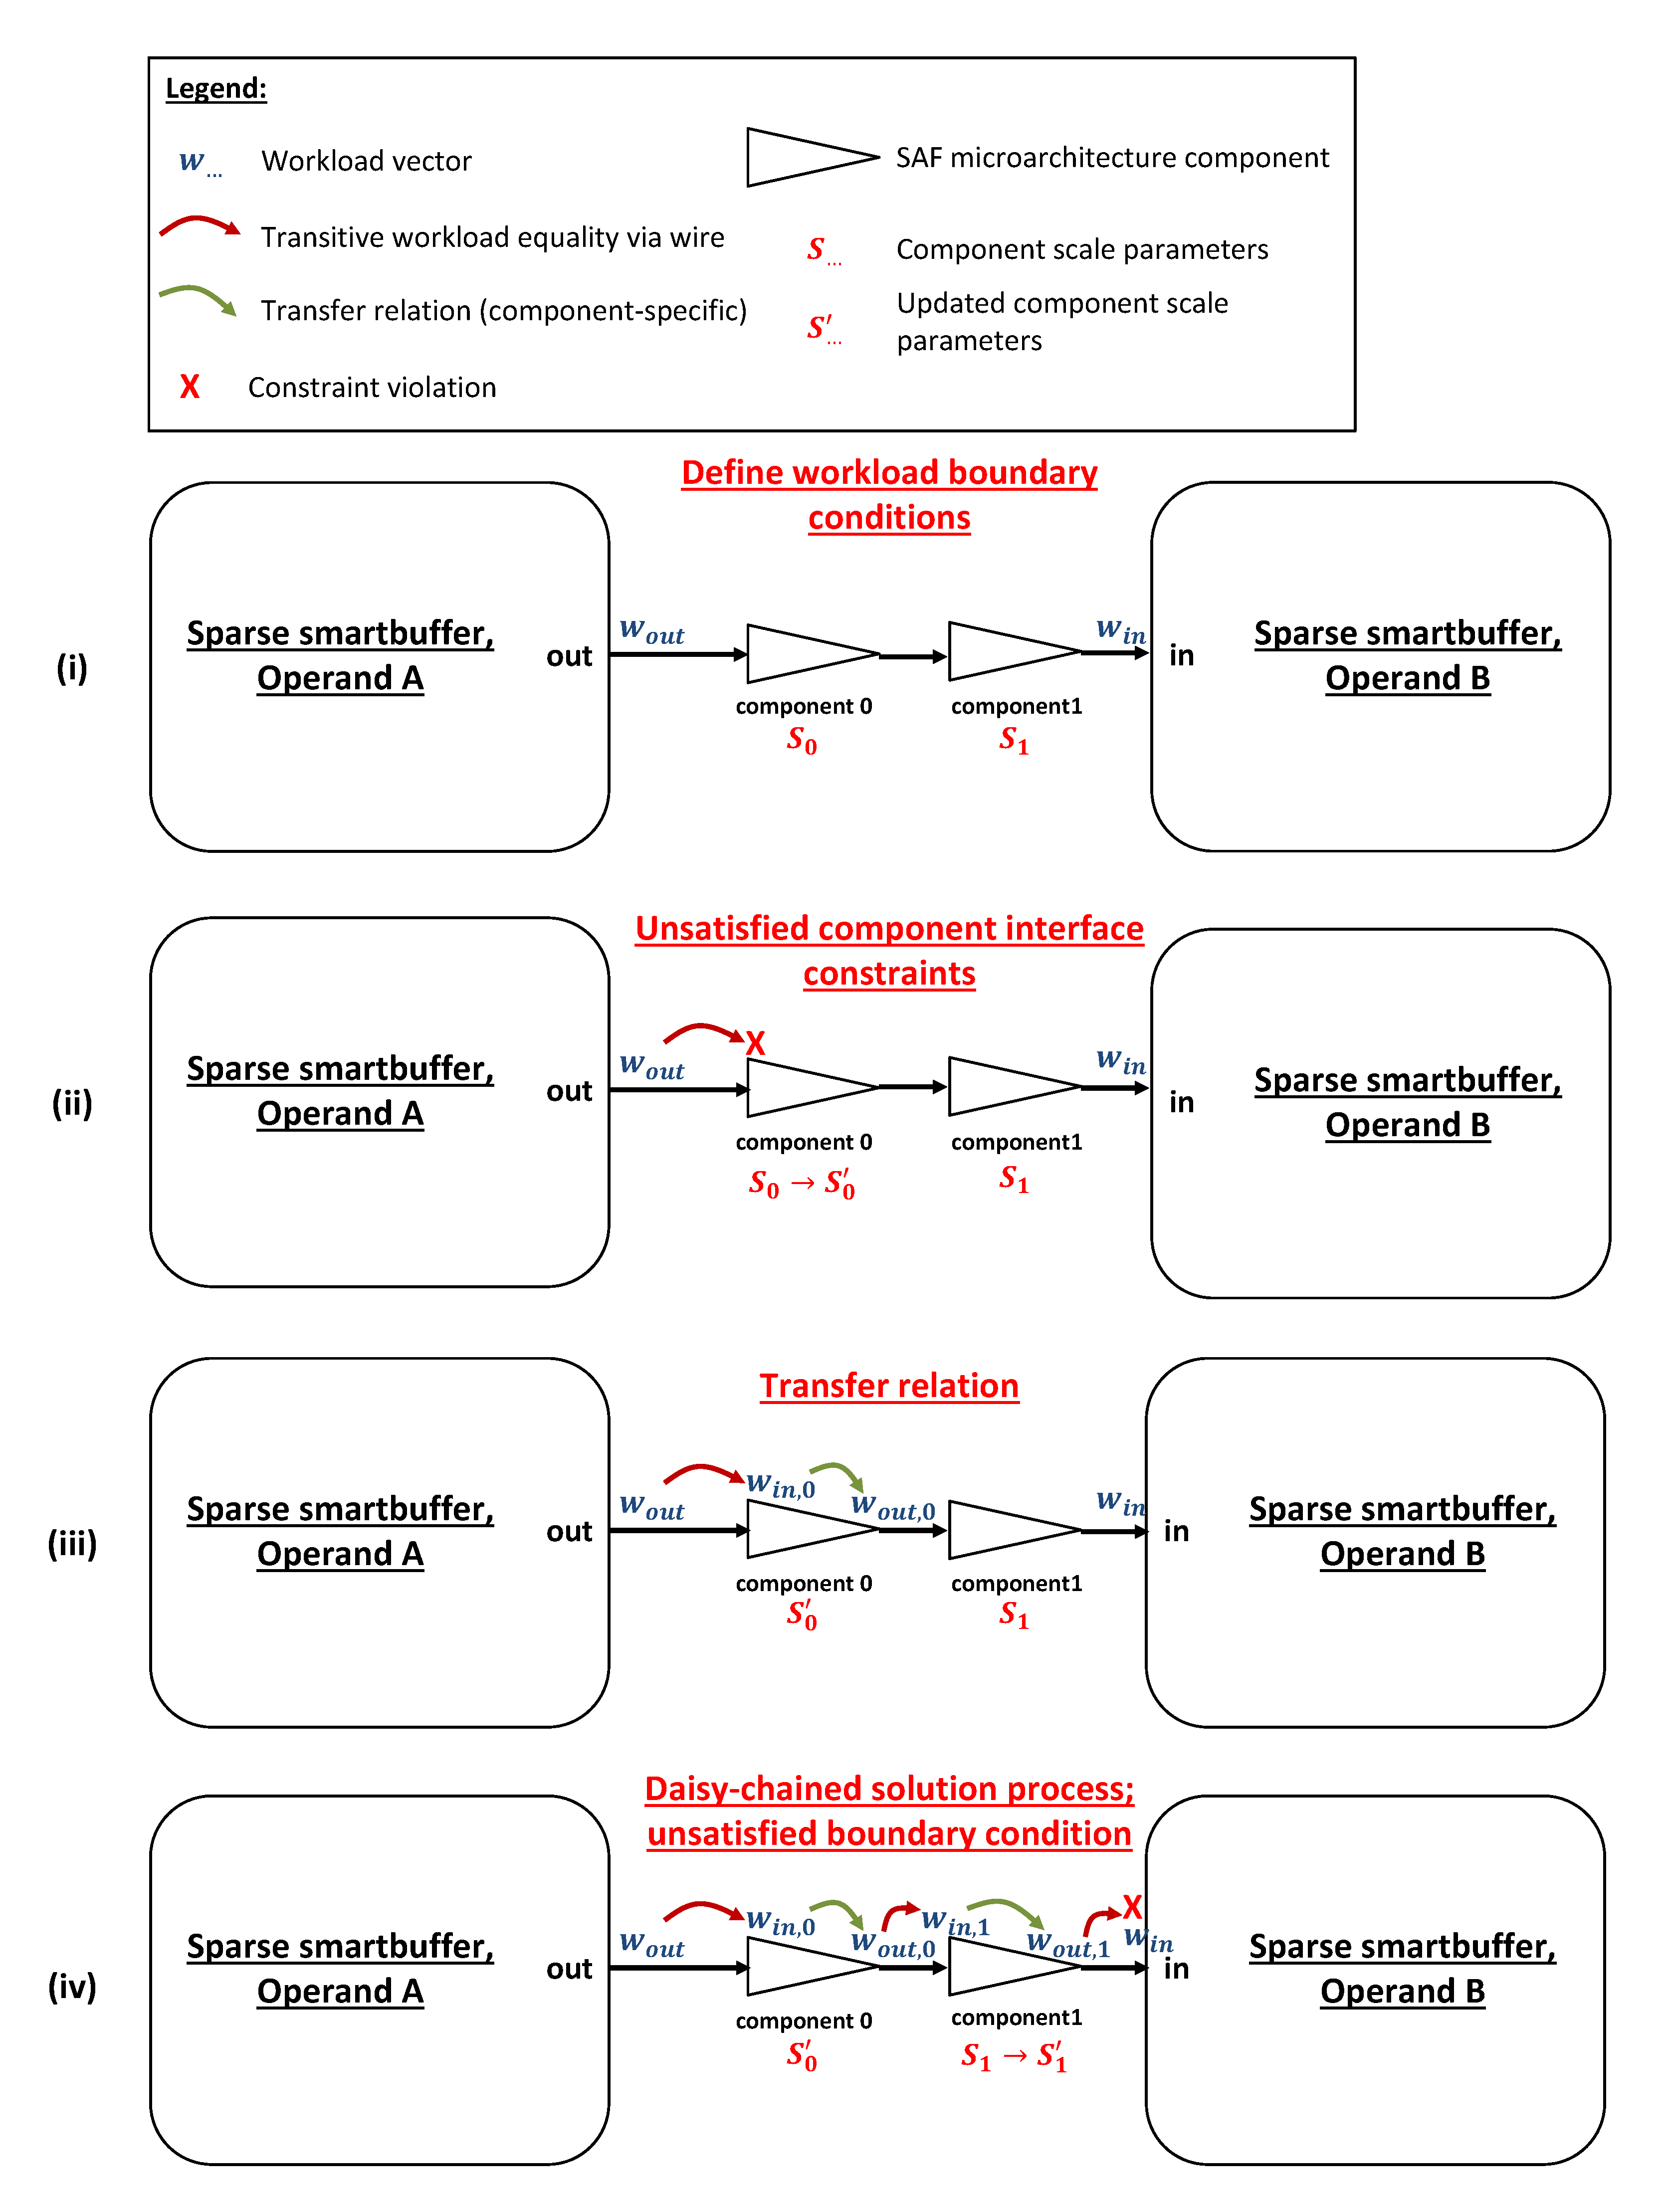
\includegraphics[width=0.8\textwidth]{figures/workload_example.pdf}
    \caption{Example of SAF microarchitecture scale inference, via daisy-chained workload solving.}
    \label{fig:workload_example}
\end{figure}

\begin{figure}[ht]
    \centering
    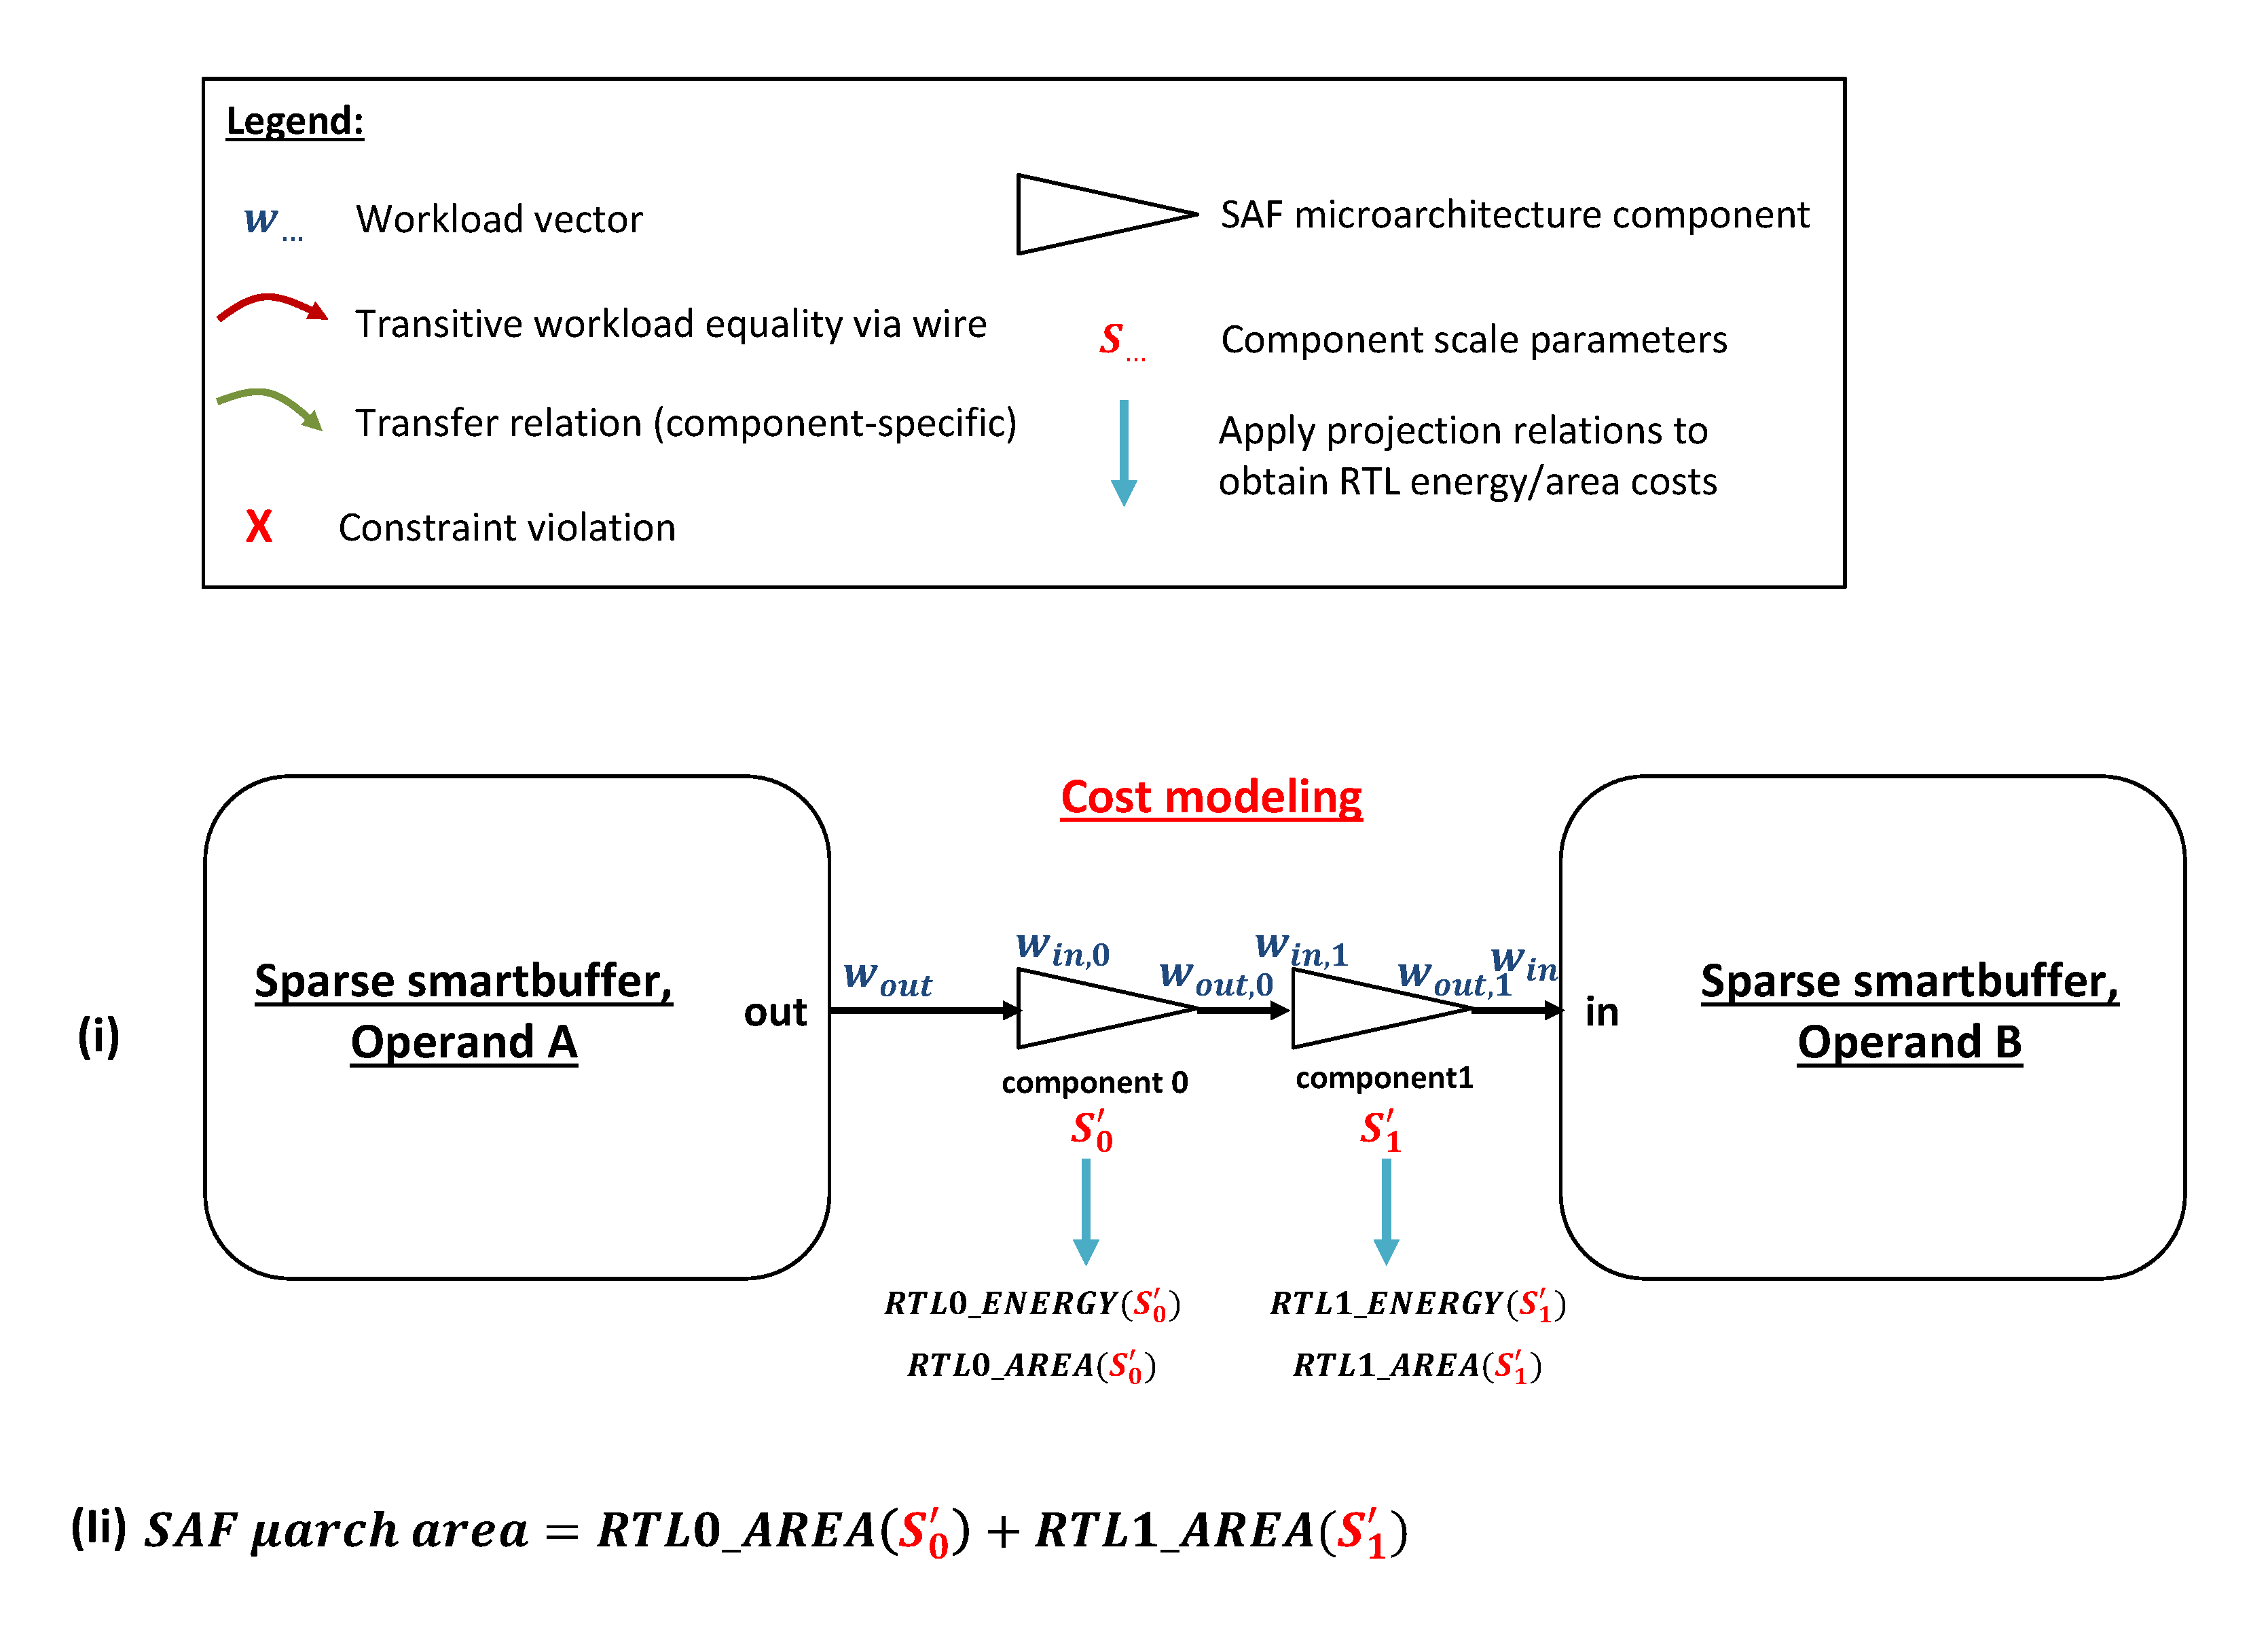
\includegraphics[width=0.8\textwidth]{figures/rtl_objective.pdf}
    \caption{Demonstration of how SAF microarchitecture scale inference makes it possible to derive values for energy and area objective functions.}
    \label{fig:rtl_objective}
\end{figure}

For modeling purposes, a SAF microarchitecture primitive model may be described entirely in terms of:

\begin{itemize}
    \item \textbf{RTL blocks -} A list of RTL modules or ``blocks'' from Chapter~\ref{chapter:rtl} which comprise the component being modeled. Figure~\ref{fig:rtl_objective} reflects that each SAF microarchitecture component may be associated with zero or more characterized RTL components. When the user defines the model of a SAF microarchitecture primitive, they must specify the list of related RTL blocks explicitly.
    \begin{itemize}
        \item \textbf{RTL parameters -} Each RTL block has zero or more parameters which customize the digital logic implementation as a function of the parameter values. RTL parameter values also impact the energy and area cost of a component. The notation for a given RTL parameter is $rtl\_name.param\_name$
        \item \textbf{Example -} A coordinate-payload-format\cite{sparseloop}\cite{szebook} intersection unit\cite{extensor} may (within the context of this work) be constructed out of EXACTLY ONE OF the following RTL blocks defined in Chapter~\ref{chapter:rtl}: a two-fingered intersection unit\cite{extensor}, a skip-ahead intersection unit\cite{extensor}, or a direct-mapped intersection unit.\cite{extensor} (of course the modeling library could be extended to support other options derived from the literature.) The input vectorization parameter of an intersection unit $isect$ would be represented notationally as $isect.md_in_vectorization$.
    \end{itemize}
    \item \textbf{Scale parameters -} A set of parameters which determine the component's load-handling capability. Figure~\ref{fig:workload_example} shows that each component is associated with a vector of scale parameter values. \textbf{Critically, scale parameters are distinct from taxonomic attributes} - taxonomic attributes are high-level characteristics which reflect choices about algorithm or scaling behavior; once the taxonomic attributes have been specified, \textit{scale parameters represent the low-level design space for implementing the particular taxonomic description.}
    \begin{itemize}
        \item \textbf{Notation -} $S_x$ is the vector of scale parameters for component $x$.
        \item \textbf{Example -} The scale parameters of a prefix-sum unit are (1) its \textbf{word bitwidth}, and (2) its \textbf{degree of vectorization}. The prefix-sum unit cannot sum a vector which is larger than its vector scale parameter. It cannot correctly sum a vector with words which have more bits than the prefix-sum unit's word bitwidth scale parameter.
    \end{itemize}
    \item \textbf{Constitutive relations -} A component is uniquely described by its energy, area, and workload models. The component's \textit{constitutive relations} define a unique set of relationships between these quantities; the constitutive relations should express an intuition about how the component functions, with specific characterized cost (energy/area) metrics for RTL blocks. Constitutive relations are specified at the time when the user writes a SAFTools model. \textbf{The key constitutive relations are:}
    \begin{itemize}
        \item \textbf{Interface constraints.} The interface relations set \textbf{upper-bounds} on workload at each component input port (i.e. upper-bounds on each dimension of the workload vector at an input port.) This is reflected by Figure~\ref{fig:workload_example}(ii). These upper-bounds are a function of the scale parameter values $S$.
        \begin{itemize}
            \item \textbf{Notation.} $I[S](w_{port0},w_{port1},...)$ is a set of interface constraints on a set of ports' workloads, parameterized by the scale parameters $S$. Typically, $I[S]()$ imposes \textit{upper-bounds}, and upper-bounds increase as $S$ increases along any dimension. \textbf{Critically, component energy/area cost also increases as $S_{comp}$ increases along any dimension.}
            \item \textbf{Corollary.} If a component has scale parameters $S_{comp}$ and the workload applied at $port0$ violates the constraint(s) $I[S_{comp}](port0)$, one can perform ``design-space exploration'' or ``tuning'' of $S_{comp}$ in order to find the minimum-cost $S^\prime_{comp}$ for which $I[S^\prime_{comp}](port0)$ is satisfied by the workload at port0. This is represented in Figure~\ref{fig:workload_example}(ii), where the scale parameters $S_0$ are adjusted to $S^\prime_0$ such that component 0 will support its input workload.
        \end{itemize}
        \item \textbf{Transfer relations.} The transfer relations are \textbf{equations or upper-bound inequalities on output-port workload(s) as a function of input-port workload(s)}; like interface constraints, transfer relations are parameterized by scale parameters. Figure~\ref{fig:workload_example} (iii) and (iv) show how output workload values (or bounds) are derived from input workloads via transfer relations. Transfer relations capture a key intuition that \textbf{SAF microarchitecture primitives frequently exploit forms of filtering or compaction, operations which yield fewer outputs (or fewer \textit{valid outputs}) than inputs.} Critically, this means that if component 0 is loaded by the output of a smartbuffer, and component 1 is loaded by the output of component 0 (as is the case in Figure~\ref{fig:workload_example}), the workload at component 1's input port may not be the same as the workload which the smartbuffer imposes on the input port of component 0.
        \begin{itemize}
            \item \textbf{Notation.} $T[S_{comp}](w_{port\_in0},w_{port\_in1},...)$
            \item \textbf{Example.} Intersecting two compressed sparse coordinate payload fibers, with $C_0$ and $C_1$ non-zero values respectively, necessarily yields an output stream which will contain $C_{out}$ non-zero matching metadata values, where $C_{out} \leq C_0$ and $C_{out} \leq C_1$. Suppose that we know (for sake of simplicity) that $C_{out} = 0.5 C_0$. Then $T[S_{comp}](w_{port\_in0},w_{port\_in1},...)$ is a set containing two relations:

            \[w_{port\_out,pr} \leq 0.5 w_{port\_in0,pr}\]

            \[w_{port\_out,pr} \leq 0.5 w_{port\_in1,pr}\]

            where $w_{port\_out,pr}$, $w_{port\_in0,pr}$ and $w_{port\_in1,pr}$ represent the \textbf{local throughput dimension (mnemonic ``pr'')} of the $port\_out$, $port\_in0$, and $port\_in1$ interfaces, respectively.
            
            \item \textbf{Example.} If two compressed sparse fibers are being intersected, the underlying dense ranks for both fibers necessarily have the same size - and furthermore, the intersected metadata stream at the intersection unit output necessarily also maps back onto the same underlying dense rank. Thus for an intersection unit, the following transfer relations also apply:

            \[w_{port\_out,nc} = w_{port\_in0,nc}\]

            \[w_{port\_out,nc} = w_{port\_in1,nc}\]

            where the $nc$ subscript refers to the dense rank size dimension (mnemonic ``nc'') of each port's workload.
        \end{itemize}
        \item \textbf{Projection relations.} The projection re
    \end{itemize}
\end{itemize}



(1) , and (2) a set of \textit{constitutive relations}  the ``workload vector'' abstraction developed in Section~\ref{sec:loadspaces}

\subsection{Deriving loadspaces from architecture and sparse optimizations}

TODO: describe how loadspaces are derived from architecture and sparse optimizations.

    \item \textbf{The meaning of ``throughput'' is representation-dependent.} This is evident in for example the coordinate metadata intersection unit described in ExTensor\cite{TODO}, in which only non-zero values are pushed onto either of the two queues leading to the intersection unit; thus, the loading on the intersection unit is a function of individual operands' sparsities. This is also evident in a microarchitectural intersection unit within a skipping microarchitecture. Its function is tied to the sparsity of both operands. An intersection requires not just a single non-zero operand but two non-zero operands simultaneously. The probability of this occurrence is a function of both operands' distribution of non-zero values. This means that sparsity, represented in whatever appropriate way, can factor into the loading on a microarchitecture.
\end{itemize}

Thus, it is clear that a single scalar value, such as throughput, is insufficient for characterizing the loading on a microarchitecture. We must resort to a multidimensional representation of loading, which therefore means that the load handling capability of a microarchitecture is also multidimensional.

Factors which impact the loading placed by an architectural port upon a SAF microarchitecture port include

\begin{itemize}
    \item \textbf{Representation formats.}
    \item \textbf{Datatypes.} SAFmodel supports three datatypes for microarchitecture ports - metadata, address, and flag. The word-width dimension of the loadspace must reflect the datatype at the applicable interface port.
\end{itemize}

\subsection{User-defined microarchitecture scale spaces}

TODO: describe how microarchitecture library must include user-specified scale-space and transfer-function descriptions.

\subsection{Continuity}

Now, consider the case of a microarchitecture with an interface that is connected to a buffer as shown in Figure~\ref{todo}.

Suppose that the microarchitecture has two scale space ranks as determined by its RTL, and the buffer interface has a load space with two ranks, perhaps indicating the sparsity and the data width.

A wire connects the interface on the buffer to the interface on the microarchitecture. So by continuity, the load space at the buffer interface is also the load space at the interface of the microarchitecture.

\subsection{Load-handling constraints}

We say that the microarchitecture can \textit{handle} the load space if for all ranks $r$ in the load space, the corresponding scale space rank $s$ satisfies $s \geq r$.

Define a point $P_L$ in the load space as an ordered pair of dimensions, where $n$ is the number of dimensions. We have a mapping $M$ that takes a load space point $P_L$ and produces a scale space point $P_S$, which is an ordered pair of scale space rank values. Let $P_{L \rightarrow S}$ represent the mapped load space point. For each dimension, it must hold that every dimension of $P_S$ is greater than or equal to the corresponding dimension of $P_{L \rightarrow S}$. Formally, if $P_S = (s_1, s_2, \ldots, s_n)$ and $P_{L \rightarrow S} = (l_1, l_2, \ldots, l_n)$, then for each $i$, $s_i \geq l_i$.

In other words, the projection of the load space point into scale space must lie within the feasible region defined by the scale space inequality.

\subsection{Circuits}

\subsection{Constructing energy and action objective functions}



\subsection{Component composition}

Now, one challenge in defining primitive components is that often they're comprised of more than one RTL block, and so we need a way to define scale space for an entire primitive component that is built out of multiple RTL blocks.

To do this, we can define a scale space for the whole component and then take note of what are the individual scale spaces of the RTL blocks comprising the components, and then based on an intuition about how the larger component interacts with the sub-components, we can define a set of mappings from the scale space of the whole component to the scale spaces of each of its RTL blocks.

Returning to the previous example where we had a component connected by a wire to a buffer and we defined an inequality relating the component scale space to the load scale space and we said that the load space projection into scale space must fall within the feasible region of the inequality. Now what we can do is use the mappings from the component scale space to the RTL scale spaces in order to project the inequality onto the RTL scale spaces and this then allows us to define inequalities between the RTL scale spaces and the load space terms of the buffer.

\subsection{Building an MINLP optimization problem}

Applying this process to the topology of an entire architecture, we are able to obtain a large set of inequalities which define the feasible regions for all of the RTL blocks comprising all of the microarchitectural components. And then we can set up a mixed-integer nonlinear program problem which tries to simultaneously solve for a set of all load spaces that is compatible with some assignment of scale space points to all components. The solution to this problem allows us to determine the scaling of all microarchitecture components in the design.

\section{Modeling intersection units}

\begin{figure}[ht]
    \centering
    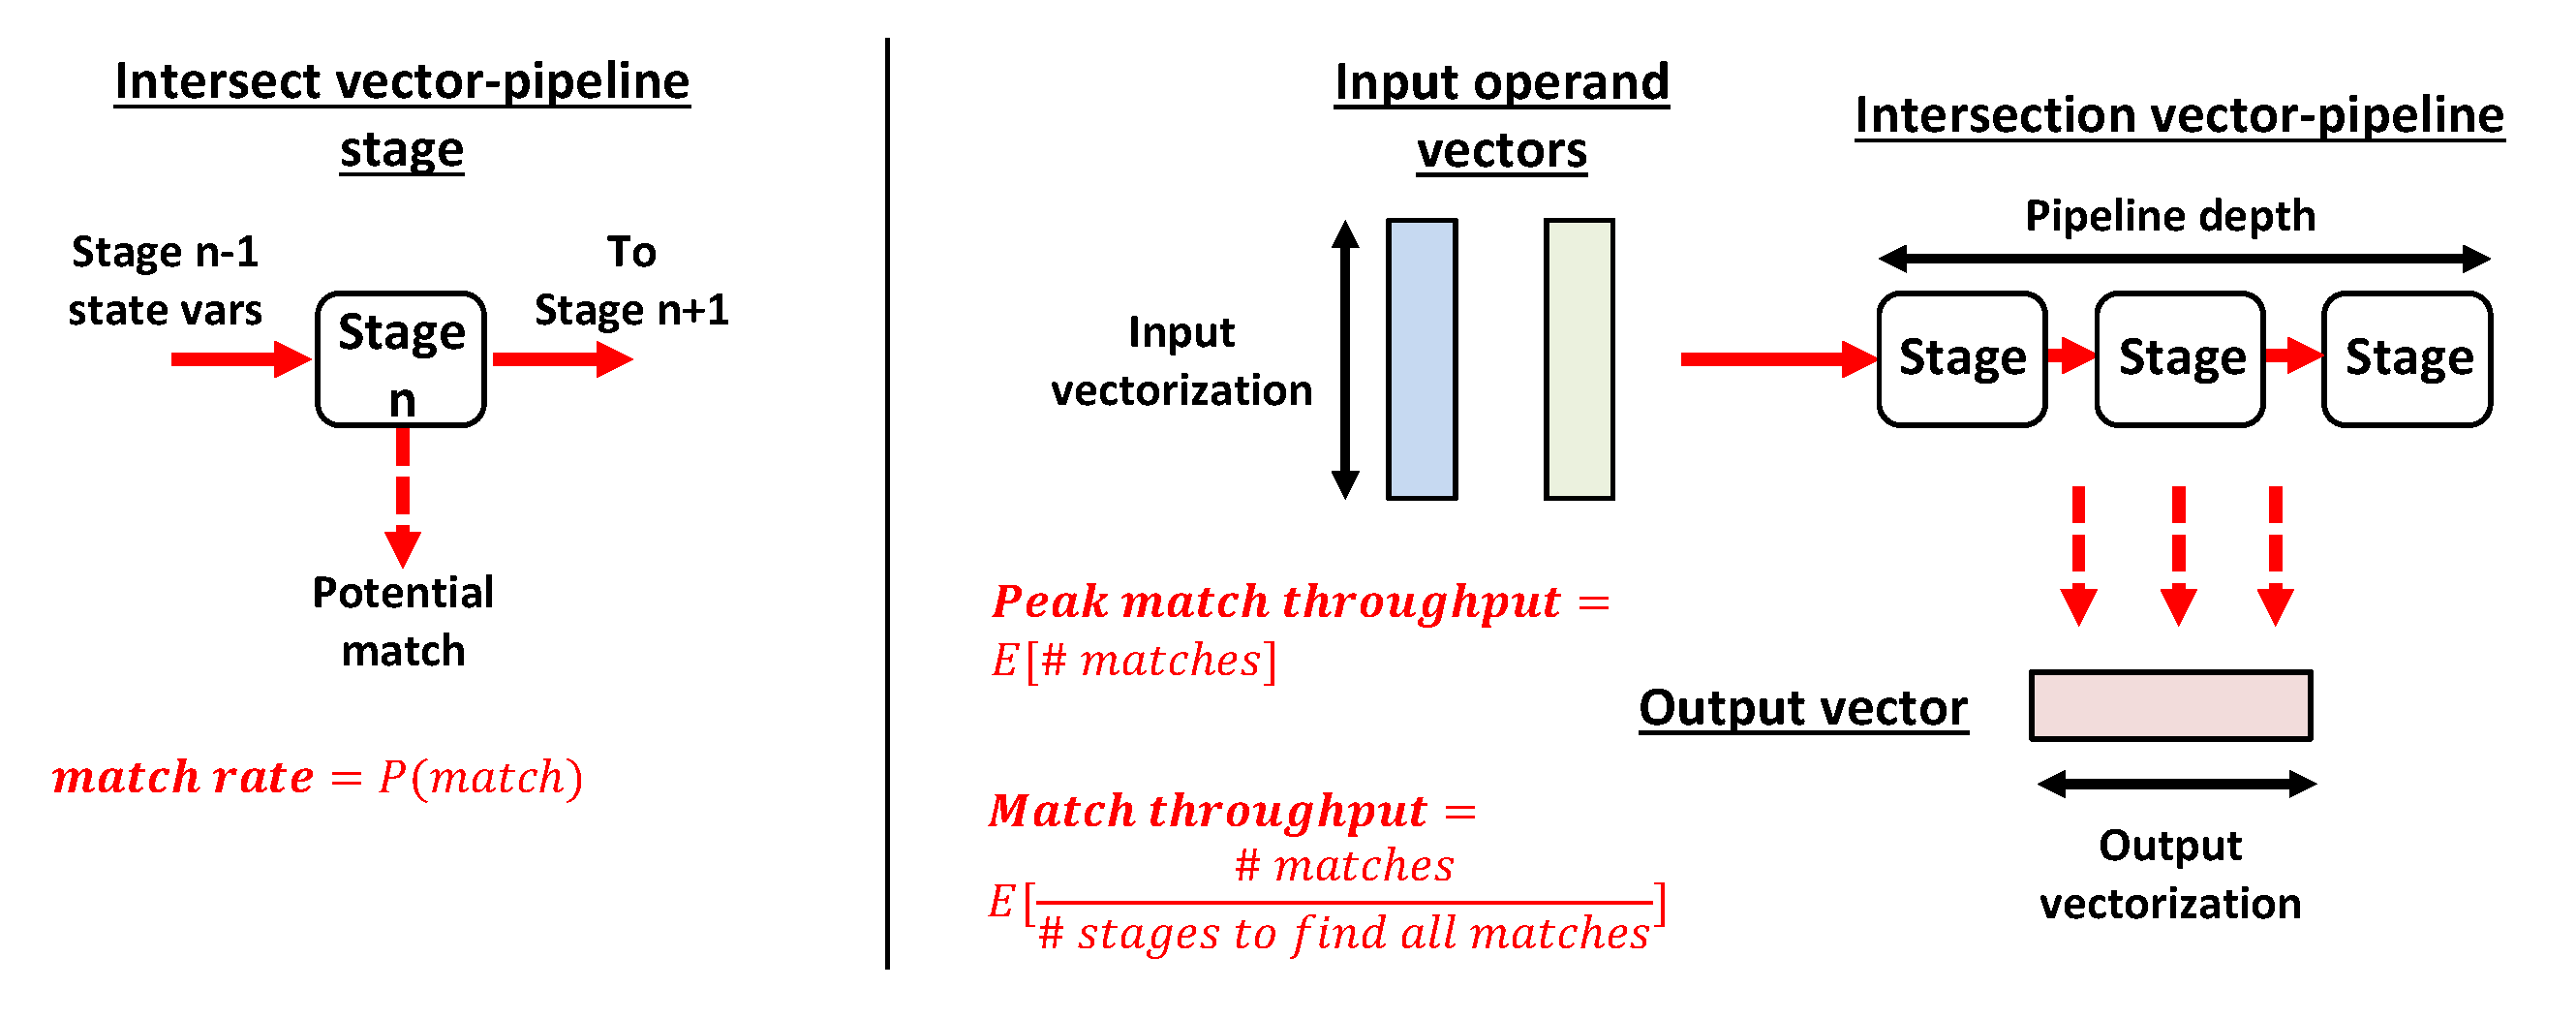
\includegraphics[width=0.95\textwidth]{figures/isect_model.pdf}
    \caption{Diagram of the relationship between the scale parameters of a vector-pipelined intersection unit (vectorization, vector-pipeline depth), and the match throughput.}
    \label{fig:isect_model}
\end{figure}

\begin{figure}[ht]
    \centering
    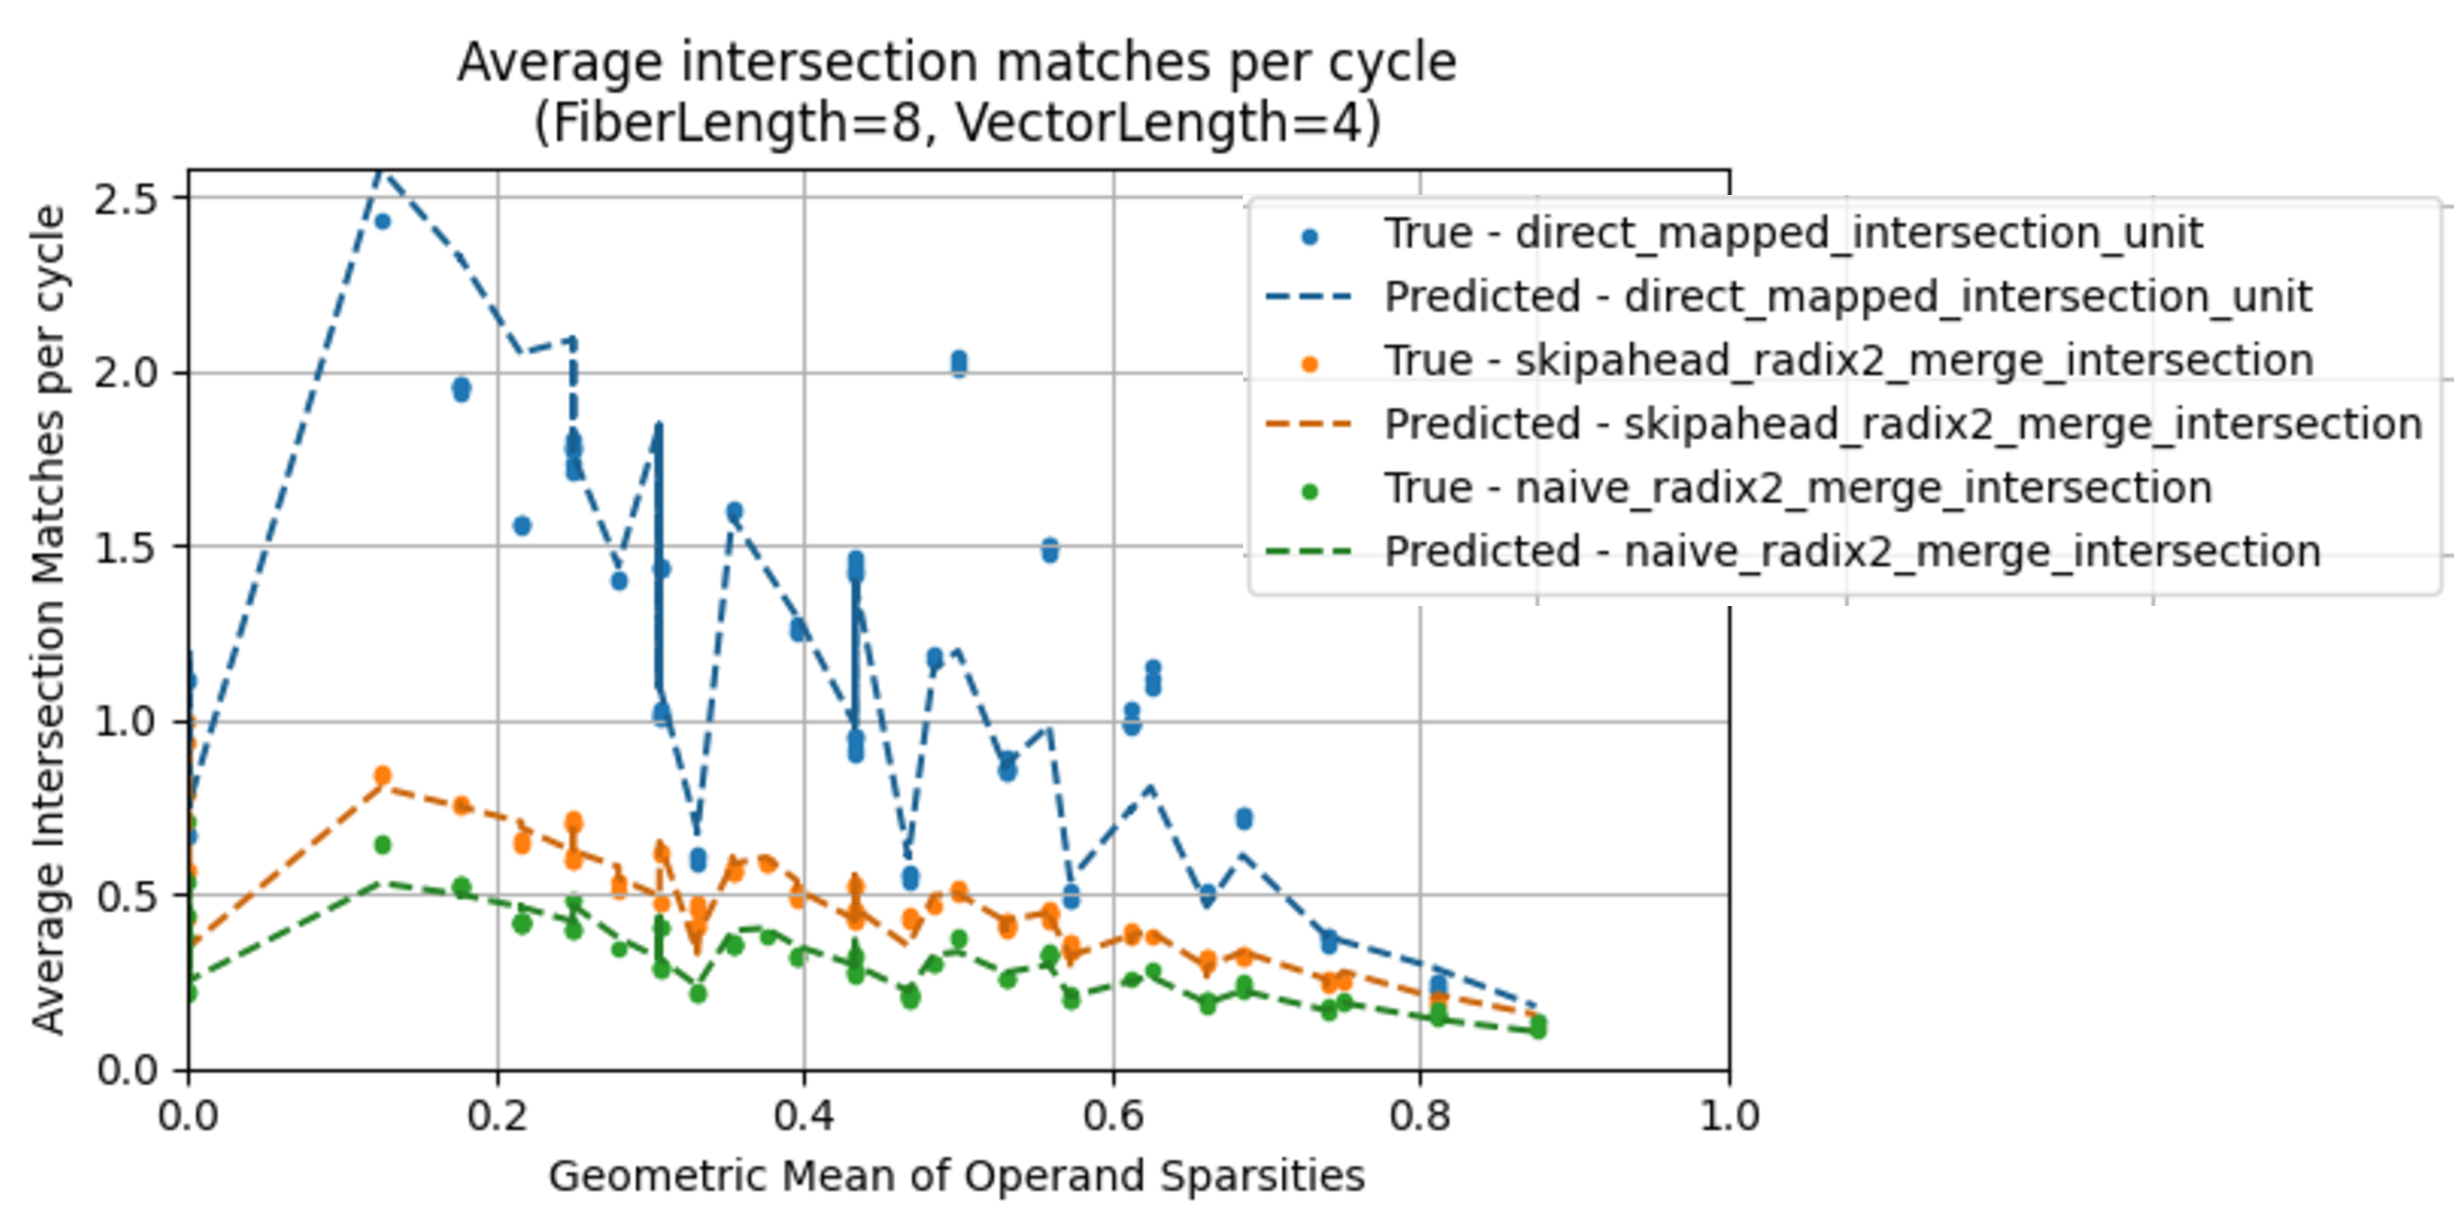
\includegraphics[width=0.95\textwidth]{figures/isect_model_fl8_vl4.pdf}
    \caption{Comparison of match throughput with respect to sparsity (geomean) for fiber size 8 and input vectorization 4. The predicted match throughput values from the analytical model developed for this work, are overlaid on simulated measurements from the intersection unit cycle accurate simulators.}
    \label{fig:isect_model_fl8_vl4}
\end{figure}